\documentclass{article}

\usepackage[accepted]{icml2022}
\usepackage{ctex}
\usepackage{graphicx}
\usepackage{booktabs}
\usepackage{hyperref}

\icmltitlerunning{MAPPO 与 HAPPO 在 SMAC 上的复现实验}

\begin{document}

\twocolumn[
\icmltitle{MAPPO 与 HAPPO 在 SMAC 上的复现实验}

\begin{icmlauthorlist}
\icmlauthor{姓名}{student}
\end{icmlauthorlist}

\icmlaffiliation{student}{学号：待填写}
\icmlcorrespondingauthor{姓名}{email@example.com}

\icmlkeywords{Multi-Agent Reinforcement Learning, SMAC, MAPPO, HAPPO}

\vskip 0.3in
]

\begin{abstract}
本文基于 HARL 代码库和 SMAC 环境，复现并比较 MAPPO 与 HAPPO 在 \texttt{3s5z} 和 \texttt{8m\_vs\_9m} 两个地图上的训练表现。报告将补充算法原理、核心代码对应、环境配置过程、win rate 曲线和实验分析。
\end{abstract}

\section{引言}

星际争霸多智能体挑战（SMAC）提供了完全合作的多智能体微操任务，适合评估多智能体强化学习算法的协同决策能力。本作业关注 MAPPO 与 HAPPO 在 SMAC 上的训练、测试和分析流程。

\section{算法概述}

\subsection{MAPPO}

MAPPO 可以理解为将单智能体 PPO 扩展到多智能体合作场景：每个智能体执行去中心化策略，训练阶段使用集中式信息估计价值函数，并通过 PPO clipped surrogate objective 限制策略更新幅度。

\subsection{HAPPO}

HAPPO 在异质智能体场景下引入顺序策略更新。其核心思想是使用多智能体优势分解，并在更新当前智能体时通过 factor 修正前序智能体策略更新对联合策略概率比的影响，从而获得更稳定的单调改进性质。

\section{HARL 代码对应}

\begin{table}[h]
\centering
\caption{论文概念与 HARL 实现对应}
\begin{tabular}{lll}
\toprule
概念 & 文件 & 位置 \\
\midrule
HAPPO clip & \texttt{happo.py} & actor update \\
HAPPO factor & \texttt{on\_policy\_ha\_runner.py} & sequential update \\
GAE & \texttt{on\_policy\_critic\_buffer\_ep.py} & compute returns \\
MAPPO update & \texttt{mappo.py} & actor update \\
SMAC win rate & \texttt{smac\_logger.py} & progress.txt \\
\bottomrule
\end{tabular}
\end{table}

更详细的文件和行号记录见 \texttt{logs/code\_reading.md}。

\section{环境配置}

本节待根据 \texttt{logs/setup.md} 和实际安装日志补充。当前已确认本机具备 NVIDIA GeForce RTX 5090，但尚未安装专用 PyTorch/HARL/SMAC 环境，且 \texttt{SC2PATH} 尚未设置。

\section{实验设置}

实验矩阵包括 MAPPO 与 HAPPO 在 \texttt{3s5z} 和 \texttt{8m\_vs\_9m} 上的训练。HAPPO 使用 HARL 官方 tuned config；由于当前 HARL commit 缺少这两个地图的 MAPPO tuned config，MAPPO 暂基于同地图 HAPPO tuned config 生成，并切换为 MAPPO 的参数共享和固定顺序设置。

\section{结果与分析}

目前已完成 1000 environment steps 的 smoke test，用于验证环境、训练脚本、日志收集和绘图流程。由于步数很少，所有实验的 eval win rate 仍为 0，因此这些曲线不能作为最终算法性能结论。

\begin{figure}[h]
\centering
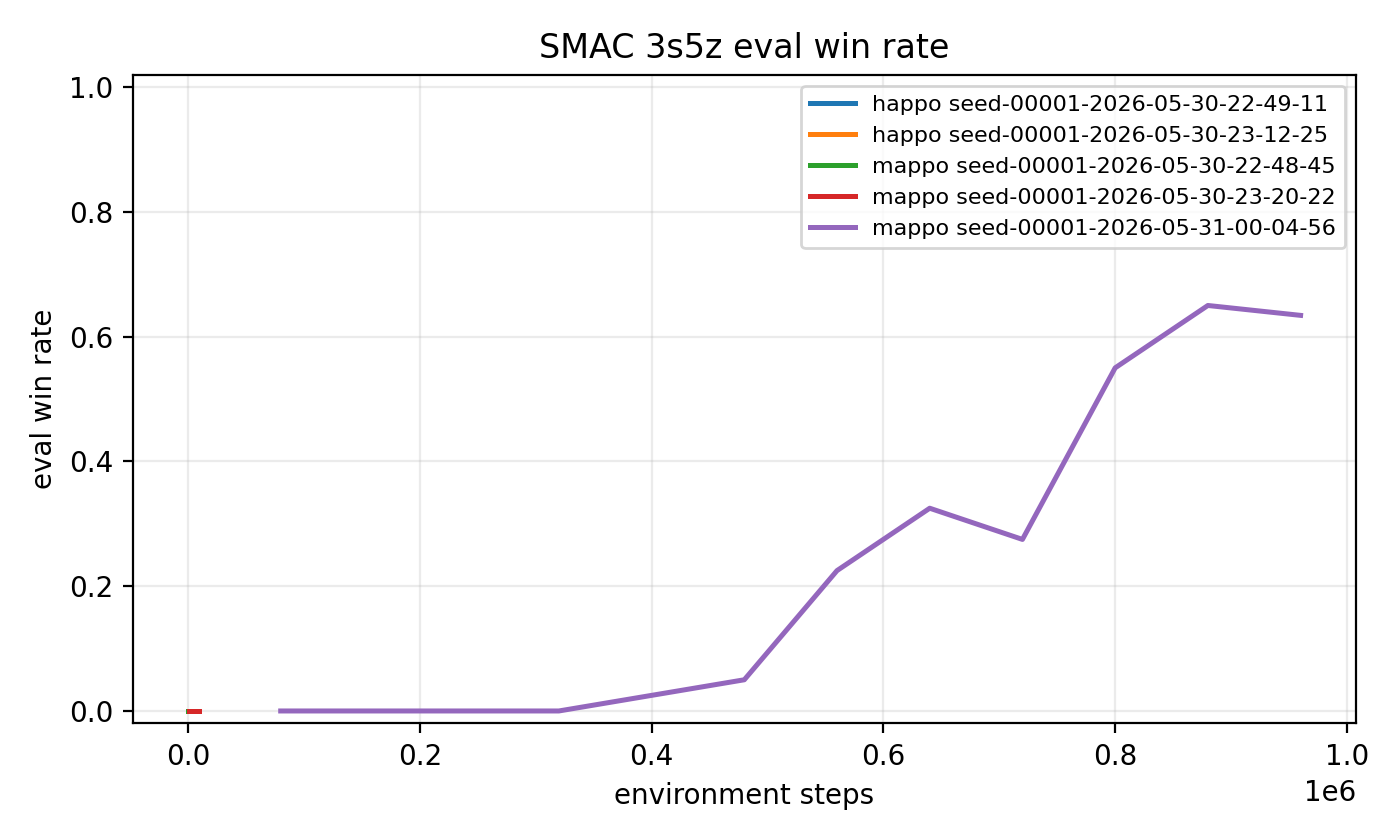
\includegraphics[width=\linewidth]{../figures/win_rate_3s5z.png}
\caption{\texttt{3s5z} smoke test eval win rate。}
\end{figure}

\begin{figure}[h]
\centering
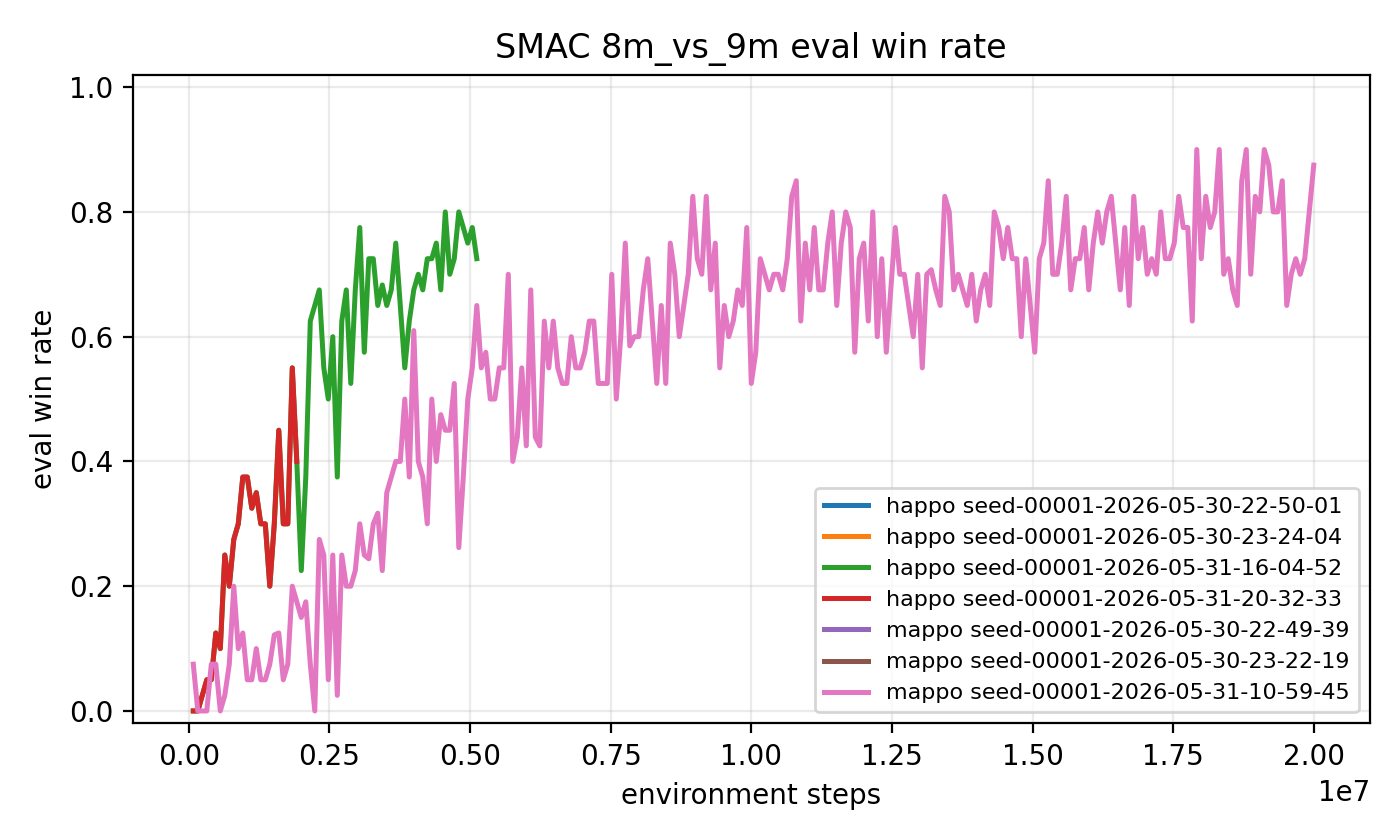
\includegraphics[width=\linewidth]{../figures/win_rate_8m_vs_9m.png}
\caption{\texttt{8m\_vs\_9m} smoke test eval win rate。}
\end{figure}

正式训练完成后，应使用相同脚本重新生成曲线，并重点比较 MAPPO 与 HAPPO 的收敛速度、最终胜率和训练稳定性。

\section{结论}

待实验完成后总结 MAPPO/HAPPO 的收敛速度、最终胜率、稳定性差异和资源限制。

\bibliography{references}
\bibliographystyle{icml2022}

\end{document}
